\section{Dataset}
The dataset chosen for training the CNN was initially found on Kaggle.com \cite{kag_set}, but was originally provided by an unknown Roboflow user on Roboflow.com \cite{rob_set}.
The dataset is licensed under CC BY 4.0, which means "Freedom to Share and Adapt".
It contains 14859 greyscale images (.jpg) of different drivers in various states of attention, alongside a .csv file with the picture names and labels. The dataset is already subdivided into train validation and test data. The pictures in the dataset are labeled one out of six classes with the labels being "SafeDriving", "DangerousDriving", "SleepyDriving", "Yawn", "Drinking", and "DistractedDriving", which will be shortened in the following for readability reasons. The number of classes is imbalanced, which has to be taken into consideration in the training of the CNN. Two example pictures from the dataset can be seen in \autoref{fig:fick}.
\begin{figure}[H]
    \centering
    \begin{subfigure}[b]{0.47\textwidth}
        \centering
        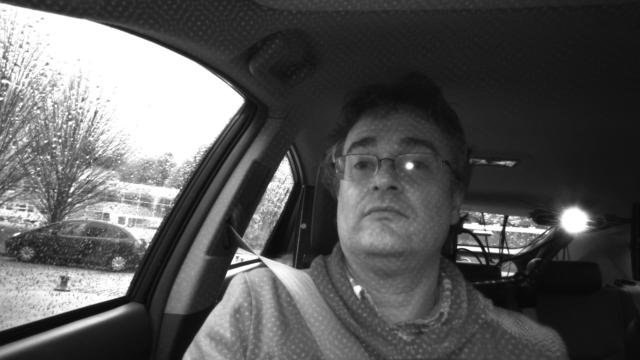
\includegraphics[width = \textwidth]{content/safe.jpg}
        \caption{Picture labeled "SafeDriving".}
        \label{fig:ggf1}
    \end{subfigure}
    \hfill
    \begin{subfigure}[b]{0.47\textwidth}
        \centering
        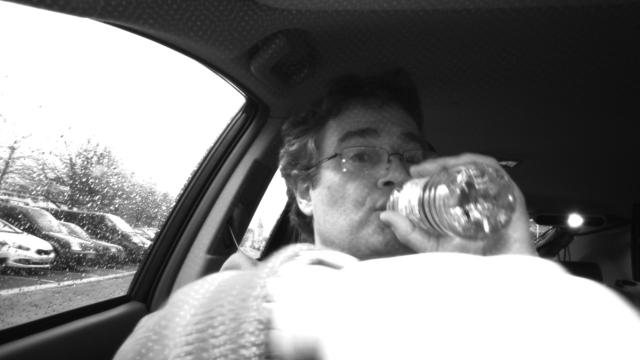
\includegraphics[width = \textwidth]{content/drinking.jpg}
        \caption{Picture labeled "Drinking".}
        \label{fig:ggf2}
    \end{subfigure}
    \caption{Two example pictures from the dataset \cite{rob_set}.}
    \label{fig:fick}
\end{figure}
\noindent
The Dataset does not contain pictures of female drivers, which might introduce a bias that is not testable in the scope of this project. The dataset was primarily chosen, due to the consistency of the pictures and its size. None of the pictures is a different format than the other or a different color channel while the camera placement and resolution are consistent throughout all data. The size of the dataset allows for more complex CNN architectures, resulting in the extraction of more subtle features and higher performance.
The dataset also comes with a pre-trained state-of-the-art object classification model, which is used as the alternative Method. The alternative model is pre-trained on the exact train test validation split that is already applied to the dataset online, which makes the comparison more convenient.